\documentclass[11pt,a4paper]{article}
\usepackage[margin=1in]{geometry}
\usepackage{kotex}
\usepackage{amsmath,amssymb}
\usepackage{booktabs}
\usepackage{hyperref}
\usepackage{enumitem}
\usepackage{array}
\usepackage{subcaption}
\usepackage{xcolor}
\usepackage{tikz}
\usetikzlibrary{arrows.meta,positioning,calc,fit,shapes.geometric,matrix,backgrounds}
\usepackage{listings}

\lstset{
  language=Python,
  basicstyle=\ttfamily\scriptsize,
  commentstyle=\color{green!40!black},
  keywordstyle=\color{blue!70!black},
  stringstyle=\color{orange!60!black},
  showstringspaces=false,
  columns=fullflexible,
  keepspaces=true,
  frame=single,
  breaklines=true
}

\title{Hands-On Graph Neural Networks Using Python\\Chapter 3 상세 정리}
\author{A7610 그래프신경망특론}
\date{\today}

\begin{document}
\maketitle
\tableofcontents
\newpage

\section{Chapter 3 개요}

Chapter 3의 목표는 그래프의 각 노드를 \textbf{고정 길이 벡터}로 바꾸는 것이다. 이렇게 얻은 노드 임베딩은 이후 분류, 링크 예측, 검색, 군집화 같은 다양한 태스크의 입력 특징으로 사용할 수 있다.

이 장의 핵심 메시지는 간단하다.
\begin{quote}
텍스트에서 단어의 문맥을 학습하는 Word2Vec의 아이디어를 그래프의 random walk 시퀀스에 적용하면, 비지도 방식으로 유용한 노드 표현을 만들 수 있다.
\end{quote}

실습 노트북 \texttt{practice/hands\_on\_gnn\_examples/Chapter03/chapter3.ipynb} 역시 이 흐름을 그대로 따른다.
\begin{enumerate}[leftmargin=*]
  \item 작은 텍스트 예제로 Word2Vec 임베딩 감각 익히기
  \item 그래프에서 random walk 생성하기
  \item Karate Club 그래프에서 DeepWalk 임베딩 학습하기
  \item t-SNE와 분류기로 임베딩 품질 확인하기
\end{enumerate}

\section{Word2Vec에서 출발하는 이유}

\subsection{분산 표현(distributed representation)}
전통적인 one-hot 인코딩은 각 단어를 서로 완전히 독립적인 기호로 취급한다. 반면 임베딩은 각 단어를 연속 벡터로 표현하고, 비슷한 문맥에서 등장하는 단어는 비슷한 벡터를 갖도록 학습한다.

\[
\text{one-hot word} \rightarrow \text{dense vector embedding}
\]

이 관점은 그래프에서도 그대로 유효하다. 노드를 단순 정수 ID로 두면 구조적 유사성을 직접 표현할 수 없지만, 임베딩 벡터로 바꾸면 ``어떤 노드가 어떤 역할과 주변 문맥을 갖는가''를 수치화할 수 있다.

\subsection{Skip-gram 목적}
Word2Vec의 skip-gram 모델은 중심 단어가 주변 단어를 잘 예측하도록 학습한다.

\[
\max \sum_{t=1}^{T} \sum_{-c \le j \le c, j \neq 0} \log p(w_{t+j}\mid w_t)
\]

여기서 중요한 것은 정확한 확률식 자체보다도, \textbf{문맥을 공유하는 토큰들이 가까운 벡터를 갖게 된다}는 점이다.

\subsection{노트북의 첫 실습}
노트북 초반부는 텍스트 말뭉치에 대해 아래와 같이 Word2Vec을 학습한다.

\begin{lstlisting}
model = Word2Vec([text],
                 sg=1,
                 vector_size=10,
                 min_count=0,
                 window=2,
                 workers=1,
                 seed=0)
\end{lstlisting}

이 단계는 단순 예제이지만 매우 중요하다. DeepWalk는 완전히 새로운 모델이라기보다, \textbf{입력 데이터를 텍스트 문장에서 그래프 walk로 바꾼 Word2Vec 응용}이기 때문이다.

\section{Random Walk를 문장으로 보기}

\subsection{그래프 시퀀스 생성}
그래프에서 문장에 해당하는 것은 노드 방문 시퀀스다. 가장 단순한 방법은 random walk이다.

\begin{figure}[h]
\centering
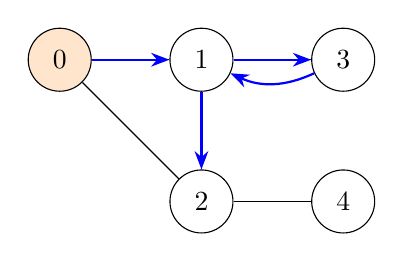
\begin{tikzpicture}[>=Stealth,node distance=1.8cm]
\tikzstyle{n}=[circle,draw,minimum size=8mm]
\node[n,fill=orange!20] (a) {0};
\node[n,right of=a] (b) {1};
\node[n,below of=b] (c) {2};
\node[n,right of=b] (d) {3};
\node[n,right of=c] (e) {4};
\draw (a)--(b);
\draw (a)--(c);
\draw (b)--(c);
\draw (b)--(d);
\draw (c)--(e);
\draw[->,thick,blue] (a) -- (b);
\draw[->,thick,blue] (b) -- (d);
\draw[->,thick,blue] (d) to[bend left=25] (b);
\draw[->,thick,blue] (b) -- (c);
\end{tikzpicture}
\caption{한 random walk 예시: $0 \rightarrow 1 \rightarrow 3 \rightarrow 1 \rightarrow 2$}
\end{figure}

노트북 구현은 다음과 같다.

\begin{lstlisting}
def random_walk(start, length):
    walk = [str(start)]

    for i in range(length):
        neighbors = [node for node in G.neighbors(start)]
        next_node = np.random.choice(neighbors, 1)[0]
        walk.append(str(next_node))
        start = next_node

    return walk
\end{lstlisting}

\subsection{왜 random walk가 유용한가?}
\begin{itemize}[leftmargin=*]
  \item 가까운 이웃과 자주 함께 등장하는 노드는 같은 문맥을 공유한다.
  \item 커뮤니티 내부 노드는 walk 안에서 서로 자주 co-occurrence를 일으킨다.
  \item 중심성이나 역할이 비슷한 노드는 유사한 방문 패턴을 만든다.
\end{itemize}

즉, random walk는 그래프의 지역 구조를 확률적 시퀀스로 바꾸는 장치라고 볼 수 있다.

\section{DeepWalk 알고리즘}

\subsection{절차}
DeepWalk는 다음 네 단계를 따른다.
\begin{enumerate}[leftmargin=*]
  \item 그래프의 모든 노드를 시작점으로 사용한다.
  \item 각 시작점에서 여러 번 random walk를 생성한다.
  \item 생성된 모든 walk를 텍스트 말뭉치처럼 모은다.
  \item skip-gram으로 노드 임베딩을 학습한다.
\end{enumerate}

\subsection{노트북의 실험 설정}
\begin{lstlisting}
walks = []
for node in G.nodes:
    for _ in range(80):
        walks.append(random_walk(node, 10))
\end{lstlisting}

\begin{lstlisting}
model = Word2Vec(walks,
                 hs=1,
                 sg=1,
                 vector_size=100,
                 window=10,
                 workers=1,
                 seed=1)
\end{lstlisting}

여기서 하이퍼파라미터는 다음 의미를 갖는다.
\begin{itemize}[leftmargin=*]
  \item \texttt{80}: 노드당 샘플링 횟수. 많을수록 안정적이지만 비용이 증가한다.
  \item \texttt{10}: walk 길이. 더 긴 구조를 반영하지만 노이즈도 늘 수 있다.
  \item \texttt{window=10}: 한 walk 안에서 멀리 떨어진 노드도 같은 문맥으로 본다.
  \item \texttt{vector\_size=100}: 노드 표현의 차원 수다.
\end{itemize}

\subsection{이 장에서 얻는 직관}
DeepWalk는 노드 feature가 거의 없거나 전혀 없을 때에도 구조만으로 표현을 만들 수 있다는 장점이 있다. 반면 지도 신호를 직접 사용하지 않으므로, 최종 태스크에 꼭 최적인 임베딩이 되리라는 보장은 없다.

\section{Karate Club 실습 해설}

\subsection{데이터셋 의미}
Karate Club 그래프는 34개 노드의 소규모 소셜 네트워크이며, 실제 동아리 분열에 따라 두 개의 커뮤니티 라벨이 존재한다.

\begin{lstlisting}
G = nx.karate_club_graph()

labels = []
for node in G.nodes:
    label = G.nodes[node]['club']
    labels.append(1 if label == 'Officer' else 0)
\end{lstlisting}

이 데이터셋은 ``구조만으로 커뮤니티를 얼마나 복원할 수 있는가''를 빠르게 보기 좋은 예제다.

\subsection{유사 노드 검색}
학습 후에는 특정 노드와 비슷한 문맥을 가진 노드를 찾을 수 있다.

\begin{lstlisting}
for similarity in model.wv.most_similar(positive=['0']):
    print(similarity)
\end{lstlisting}

만약 노드 0과 같은 커뮤니티 안에 있는 노드들이 상위에 자주 등장한다면, 임베딩이 커뮤니티 구조를 어느 정도 반영하고 있다고 해석할 수 있다.

\subsection{t-SNE 시각화}
\begin{lstlisting}
nodes_wv = np.array([model.wv.get_vector(str(i)) for i in range(len(model.wv))])
tsne = TSNE(n_components=2,
            learning_rate='auto',
            init='pca',
            random_state=0).fit_transform(nodes_wv)
\end{lstlisting}

t-SNE는 고차원 공간의 국소 이웃 관계를 2차원으로 압축해 보여준다. 따라서 완벽한 성능 지표는 아니지만, 라벨별로 점들이 어느 정도 분리되는지 빠르게 확인하는 데 유용하다.

\subsection{분류 태스크 연결}
노트북 마지막 부분은 학습된 임베딩을 입력 특징으로 하여 간단한 분류기를 학습한다.

\begin{lstlisting}
clf = RandomForestClassifier(random_state=0)
clf.fit(nodes_wv[train_mask], labels[train_mask])

y_pred = clf.predict(nodes_wv[test_mask])
acc = accuracy_score(y_pred, labels[test_mask])
\end{lstlisting}

이 실험은 중요한 메시지를 준다.
\begin{quote}
DeepWalk 자체는 분류 모델이 아니지만, 잘 학습된 임베딩은 단순한 다운스트림 모델만으로도 좋은 예측 성능을 낼 수 있다.
\end{quote}

\section{실습과 이론을 연결해서 보기}

\subsection{노트북 셀 흐름의 의미}
\begin{enumerate}[leftmargin=*]
  \item \textbf{셀 1--3}: Word2Vec으로 임베딩 학습 감각 습득
  \item \textbf{셀 4--5}: 작은 그래프에서 random walk 생성기 확인
  \item \textbf{셀 6--8}: Karate Club에 DeepWalk 적용
  \item \textbf{셀 9--11}: 유사도, 시각화, 분류로 품질 평가
\end{enumerate}

이 순서는 교육적으로 잘 설계되어 있다. 처음부터 DeepWalk 정의를 주입하는 대신, ``왜 이 알고리즘이 작동할 것 같은가''를 Word2Vec 예제에서 먼저 체감하도록 만들기 때문이다.

\subsection{수업에서 강조하면 좋은 포인트}
\begin{itemize}[leftmargin=*]
  \item DeepWalk는 \textbf{비지도 표현학습}이다.
  \item 입력은 그래프지만 학습기는 사실상 \textbf{언어 모델 기반 임베딩 학습기}다.
  \item random walk는 그래프의 인접성, 커뮤니티, 역할 정보를 부분적으로 시퀀스로 바꿔 준다.
  \item 최종 태스크 성능은 walk 전략과 하이퍼파라미터에 크게 좌우된다.
\end{itemize}

\section{한계와 다음 장으로의 연결}

\subsection{DeepWalk의 한계}
\begin{itemize}[leftmargin=*]
  \item 단순 uniform random walk만 사용하므로 탐색 편향을 세밀하게 제어하기 어렵다.
  \item 노드 속성(feature)을 직접 활용하지 않는다.
  \item 최종 분류 목적을 직접 최적화하지 않는다.
  \item 매우 큰 그래프에서는 walk 생성과 학습 비용이 커질 수 있다.
\end{itemize}

\subsection{왜 이후에 GNN이 필요한가?}
GNN은 random walk로 우회하지 않고, 이웃 집계(message passing)를 통해 그래프 구조와 노드 특징을 함께 end-to-end로 학습한다. 즉 DeepWalk가 ``구조 기반 비지도 임베딩''의 강력한 출발점이라면, GNN은 이를 지도학습 및 feature 활용까지 확장한 일반적 프레임워크라고 볼 수 있다.

\section{Chapter 3 핵심 요약}
\begin{itemize}[leftmargin=*]
  \item DeepWalk는 random walk + skip-gram의 조합이다.
  \item random walk 시퀀스는 그래프 구조를 텍스트 문맥처럼 바꿔 준다.
  \item 학습된 노드 임베딩은 유사도 검색, 시각화, 노드 분류에 활용할 수 있다.
  \item Karate Club 예제는 구조만으로도 커뮤니티 정보가 어느 정도 복원됨을 보여준다.
  \item 이 장은 전통적 그래프 표현학습에서 GNN으로 넘어가는 중요한 다리 역할을 한다.
\end{itemize}

\end{document}
